\chapter{Theoretical Foundations}
\section{Mathematical Foundations}
When modelling we always need ways to express facts in mathematical terms. E.g from physic we know a lot of equations that express the relations between different physical values. We are often modelling in order to derive an answer to some particular question. If we are lucky there exists an algorithm and even a software implementation that can compute the answer to our question. In the following we will introduce a variety of different ways to state problems and shortly mention their implications for solvability.
\subsection{Constraint Programming}
\begin{figure}
\label{fig:CSPExample}
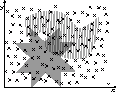
\includegraphics[width=0.5\textwidth]{./pics/SetIntersection.pdf}
\caption{Two dimensional search space and three different subsets forming a constraint satisfaction problem}
\end{figure}
In a \emph{constraint satisfaction problem} (CSP) the task is to assign values $v(x_i)$ to a set of variables $X = (x_1, \dots , x_n)$ from a free search space $S=D_1\times \dots \times D_n$ such that all relations $c_1,\dots,c_k$ between the variables hold. We call those relations $c_1,\dots,c_k$ \emph{constraints}. $D_i$ is called the domain of $x_i$, $n$ is the number of variables and $k$ the number of constraints. Mathematically we can formalise this as shown in equations \ref{CSP}ff. \cite{Eiben97constraintsatisfaction}\cite{wiki:CSP}.
\begin{eqnarray} 
\label{CSP}
c_i \subseteq S \qquad\forall i \in \left[ 1 \dots k \right]\\
\text{find:} \quad v(x_i) \in D_i \qquad\forall i \in \left[ 1 \dots n \right]| \\
\text{subject to:} \quad (v(x_1),\dots , v(x_n)) \in c_j\qquad\forall j \in \left[1 \dots k\right]
\end{eqnarray} 
Any point in $S$ within all constraints is called a \emph{feasible solution}. The set of all feasible solutions is called \emph{feasible set}. The feasible set is the intersection of all constraints. If the feasible set is the empty set we call the problem infeasible. Solving a constraint satisfaction problem means finding one feasible solution. Solving the corresponding decision problem means just to tell whether a solution exists or not. \\
Practically constraints are often specified as boolean terms over a subset of $X$ e.g. $x_1=x_2$ or even just one variable e.g. $0\leq x_1 \leq 1$. It is possible to extend any relation between $x_1$ and $x_2$ to a n-ary relation between $x_1,\dots,x_n$. In the extended relation all possible values for the variables not contained in the term specifying a relation are admitted.\\
Note also that there are in general no restrictions on the domains of the variables and the search space. It could be continuous, discrete, finite and infinite. Well known domains are integer, real, boolean but also city names or all triangles similar to an equilateral triangle could form a domain. In other literature about constraint programming often finite discrete search spaces are assumed \cite{Citation Needed}. In fact on a computer an unlimited real number is stored in IEEE 754 floating point format, which is a finite discretization of the real numbers. Also the constraints can have arbitrary properties. Even a fractal set would be acceptable as constraint.\\
In figure \ref{fig:CSPExample} we can see a two dimensional continuous search space and three sets. One that could be assembled by a union of intersections of halfspaces, another that has an arbitrary shape and the last set consists of discrete points marked by the crosses. Any of the points within the intersection of those three sets would be a solution to the corresponding CSP.\\
There is no way to handle all possible ways to describe the constraints by one single algorithm. Additionally this general form includes also a lot of problems that are known to be undecidable or just infeasible to compute. Consequently we need to look at several specializations.
%A constraint $c_j$ is a pair $<t_j,R_j>$ of a set of variables $t_j$ and a relation $R_j$. $t_j$ is a subset of X and R is defined over those variables.

\subsection{Mathematical Programming}
A \emph{Mathematical Program} or \emph{Optimization Problem} is a constraint satisfaction problem with a real valued objective function $f:S\mapsto \mathbb{R}$ and its constraints are specified in terms of functions $g_1,\dots,g_k:S\mapsto\mathbb{R}$. We call those functions constraint functions. The search space is $\mathbb{R}^n$. The task is to find any feasible point that minimizes the objective function $f$.
\begin{eqnarray}
\text{minimize:} \quad f(X)\\
\text{subject to:} \quad g_i(X)\leq 0 \qquad \forall i\in\left[1,\dots ,k\right] 
\end{eqnarray}
\begin{definition}[local optimum]
A local optimum is a feasible solution that minimizes the objective function within a neighbouring set of feasible solutions.
\end{definition}
\begin{definition}[global optimum]
A global optimum is a feasible solution that gives the minimal value for the objective function among all feasible solutions.
\end{definition}
In practice also equations are used as constraints. A $\geq$ can be replaced by $\leq$ or the right hand side is not necessarily $0$ but an arbitrary constant. All those alternative formulations are equivalent to the given formulation.
In this thesis only linear objective functions are considered. For linear objective functions that are not constant any optimum can be found on the boundaries of the feasible set. That is why we will use the word \emph{boundary value} as an equivalent for local optimum.\\
This problem formulation still includes a lot of pathological cases, but there are algorithms as well as software implementations that try to solve problems of this kind. Algorithms trying to solve this problem include heuristic search and convex approximation. The corresponding decision problem whether a solution exists or not is known to be undecidable for this class of problems consequently there can not be a deterministic algorithm always finding a solution or reporting that the problem is infeasible.
\subsection{Convex Optimization}
While there are no efficient algorithms for all optimization problems there do exist very successful methods for solving convex optimization problems\cite{Boyd04ConOpt}.
\begin{definition}[convex set]
A set $C$ in a vector space $S$ is said to be convex if, for all points $x$ and $y$ in $C$ and all $t\in\left[0,1\right]$, the point $(1-t)x+ty$ is in $C$.
\end{definition}
\begin{definition}[convex function]
We call a function f convex iff for any two values $x$ and $y$ the in-equation $ f(\theta x + (1-\theta) y)\leq \theta f(x)+(1-\theta) f(y)$ for $\theta\in \left[0,1\right] $
\end{definition}
A convex optimization problem is a mathematical program with a convex objective function and convex constraint functions. The intersection of convex sets is a convex set itself and the set ${x\in\mathbb{R}^n|g_i(x)\leq 0}$ is a convex set. Consequently the feasible set is also convex. For convex problems every local optimum is a global optimum.\\
Convex optimization problems are particularly efficient to solve with iterative descend methods like quasi newton or interior point methods.
\subsection{Linear Programs}
Within the class of convex problems there are a lot of special cases. We will only consider one special case within the convex programs, those are \emph{linear programs} (LP).
In linear programs every constraint can be represented as linear inequation and the objective function is an affine function. 
The canonical form of a linear program consists of a matrix $\mathbf{A}$ and two vectors ${c}$ and ${b}$ such that the equations \ref{linDef}f formalize the LP. The $\leq$ is evaluated component wise.
\begin{eqnarray}
\label{linDef}
\text{minimize:}\quad {c}^TX \\
\text{subject to:}\quad AX\leq{b}
\end{eqnarray}
By removing the objective function or setting ${c}={0}$ the problem is relaxed to a linear constraint satisfaction problem. Formulations containing also equations in the constraints on some components of $X$ can be transformed to an equivalent problem in the canonical form. Also a $\max$ instead of $\min$ and a $\geq$ instead of $\leq$ can be used. In practice we will use many possible formulations.\\

An example for a linear program is given in equations \ref{linExample}f.
\begin{eqnarray}
\label{linExample}
\begin{pmatrix}
1 & -2 & 3 \\
4 & 5 & 6 
\end{pmatrix}\times\begin{pmatrix}
x_1 \\ x_2 \\ x_3
\end{pmatrix} = \begin{pmatrix}
1 \\ 4
\end{pmatrix}\\
\begin{pmatrix}
0&-1&0
\end{pmatrix}\times\begin{pmatrix}
x_1 \\ x_2 \\ x_3
\end{pmatrix}\leq \vec{0}
\end{eqnarray}

For constraint satisfaction and constrained optimization with linear constraints and objective function usually an implementation of the simplex algorithm\cite{dantzig63Simplex} is used to solve it very efficiently. Although its worst case runtime is exponential the average runtime grows linear with the number of constraints.

\subsection{Boolean Satisfiability Problems}
In a classic boolean satisfiability problem (SAT) all variables are within the boolean domain and can take the values $true$ and $false$ or $0$ and $1$ respectively. The constraint relations are expressed by a boolean formula. The variables in a SAT problem are also called literals. The task is to find an assignment to the literals, that makes the formula true. A simple example for a boolean formula is given in \ref{boolFormula}.
\begin{eqnarray}
x_1 \land \neg x_2  \lor \neg x_1 \land {x_2}
\label{boolFormula}
\end{eqnarray}
Any boolean formula can be normalized to the disjunctive normal form (DNF). For SAT there is DPLL\cite{DPLL} one of the most efficient algorithms. There are instances of SAT that are NP-complete and thus are in practice infeasible to solve although the corresponding decision problem is always decidable and DPLL is deterministic.\\
An important extension of the SAT problem is the satisfiability modulo theories (SMT) problem. Here instead of literals also sentences that evaluate to true or false in some other theory can appear. Popular backround theories used for SMT are the free theory, linear arithmetic or the theory of bit vectors. In the equations\ref{eqn:SMTExample}f we see an example formula containing propositions in linear arithmetic, Integer arithmetic and one boolean literal.
\begin{eqnarray}
\label{eqn:SMTExample}
x_1,x_2\in \mathbb{R} x_3 \in \mathbb{Z} x_4\in \mathbb{B}\\
(x_1\leq 5) \land (-x_2\leq 10) \lor (x_3=2) \land x_4
\end{eqnarray}
The practicality of SMT problem formulations depend on the used background theories. The famous SMT solver CVC currently implements a large number of logical theories and their combinations\cite{cvc}.

\subsection{Properties of the Search Space}
\subsubsection{Integer Programming}
When all variables in a CSP are from a discrete domain such as finite sets or natural numbers we call it an \emph{integer program} IP. Most integer programs are NP-complete. Famous instances are the discrete logarithm problem or factorization of numbers with only two prime factors. A constraint satisfaction problem or constrained optimization problem where at least one of the domains $D_i$ is discrete among other continuous domains is called a mixed integer problem (MIP). While all linear and most convex optimization problems with only continuous domains can be solved in polynomial time, the introduction of variables with discrete domains often makes the problem much more complex. A linear program with only discrete domains is called \emph{linear integer program} (LIP) and it is a \emph{mixed linear integer program} (MILP) when it has both discrete and continuous domains. We will consider an IP or MIP whose continuous relaxation is a convex problem a \emph{convex mixed integer program}. The continuous relaxation of a mixed inter program is the mathematical program where all discrete
domains are replaced by corresponding continuous domains e.g. the set 
$\left\lbrace 1,2,3 \right\rbrace $
 is replaced by the interval 
 $\left[ 1,3 \right] $
 .\\
An example of an convex mixed integer problem can be given
\begin{eqnarray}
x_1,x_2\in \mathbb{Z} x_3\in \mathbb{R}\\
\text{minimize:}\quad x_3 \\
\text{subject to:}\quad x_1^2 + x_2^2 - 10.5 + x_3 \leq 0 \\
\text{subject to:}\quad x_3 \geq 0
\end{eqnarray}
one possible solution to this problem is $x_1=1$ and $x_2=3$ and the optimal value for $x_3$ is $0.5$. Without the constraint $x_1$ and $x_2$ being Integers it would be easy to find assignments for those variables such that $x_3$ is $0$.\\
Strategies to solve mixed integer programmes include solving its continuous relaxation and do some sort of backtracking as e.g in branch and bound or branch and cut.
\subsubsection{Finite Search Spaces}
When each domain is a finite set then the search space is also finite. In this case at least theoretically one can always find a solution or deny the existence of a solution after exhaustive search. In practice it can still happen that the search space is finite but too large for exhaustive search.\\
%The class of mathematical programs contains instances whose decision problems are undecidable.
%In general CSPs with infinite domains and nonlinear algebraic constraints are undecidable. 
%There are some heuristic algorithms capable of solving many instances of those problems. There exist problem instances for which algorithms tend to run forever. 
One option to break down problems with continuous or infinite search space is reducing its search space to a finite discrete set of possible values. This excludes the largest portion of the search space but makes the problem handleable with existing constraint programming systems. This technique is called \emph{bounded model checking}. This concept matches pretty well with the fact that a computer can only encode finite sets. It is suitable to find a solution if there is one but if it does not find a solution it is not a guarantee that the original problem does not have a solution.\\
Finite constraint programs are usually solved by reducing the domains of variables by constraint propagation and backtracking. Examples for working constraint programming systems are B-Prolog and SWI-Prolog\cite{citation needed}. A well known bounded model checker is SMV\cite{citation needed}. 


\section{UML}
The Unified Modelling Language (UML \texttrademark ) is a graphical modelling language defining 13 different diagrams that can be used to describe the architecture, behaviour and interaction of a software systems. Modelling Elements of the UML are defined via the Meta Object Facility (MOF). Any Diagram is internally stored in a Machine readable fashion; this makes it suitable for more than just documentation purpose. With precise modelling a UML Model can also be executed or otherwise automatically analysed. In our case we want to use it to derive necessary test code for C-functions from their corresponding UML Activity Model. \\ We are using only a small subset of the complete UML here for this thesis. The figure \ref{relevantUMLClassDiagram} shows an overview of the most relevant UML modelling elements and their associations in a UML class diagram. We need to understand those elements and their relationships with each other. In the next chapters whenever referring to an element of the UML it will be printed in a special font such as \UMLType{Class}. When we refer to a reference element in UML we will put it into another special font for Example: \UMLReference{ownedOperations}.
\begin{figure}\label{relevantUMLClassDiagram}
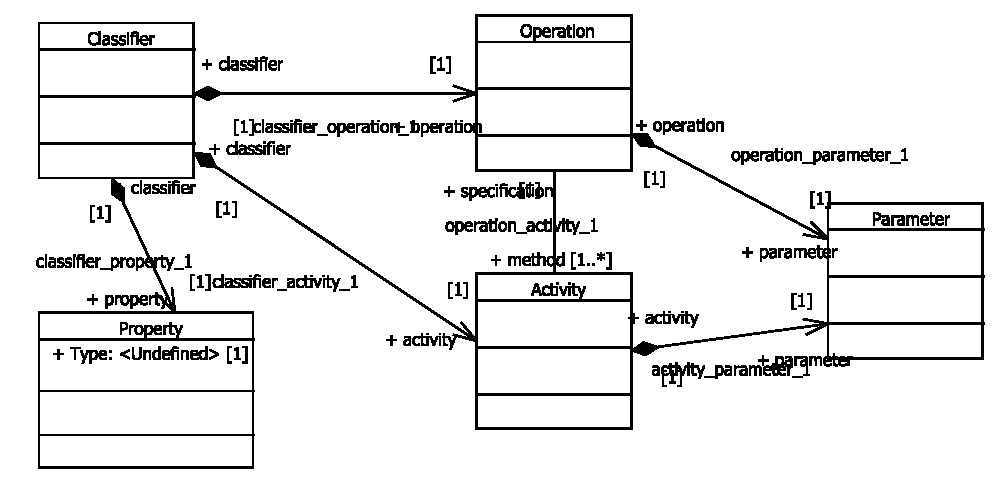
\includegraphics[width=\textwidth]{./pics/relevantUML.pdf}
\caption{Class Diagram of UML Elements used for Modelling}
\end{figure}
\subsection{Structural Modelling Elements}
\subsubsection{Package}
Packages or Namespaces are concepts that are well known to Java or C++ programmers. UML provides Packages for partitioning large Software projects. In the UML Specification we read:
\begin{quotation}
A package is used to group elements, and provides a namespace for the grouped elements.
A package is a namespace for its members, and may contain other packages. Only packageable elements can be owned
members of a package. By virtue of being a namespace, a package can import either individual members of other
packages, or all the members of other packages.
In addition a package can be merged with other packages.
\end{quotation}\cite{UML23Superstructure}
\subsubsection{Class}
The concept of classes is also pretty well known from Object Oriented Programming. In the UML specification a class is described as:
\begin{quotation}
A class describes a set of objects that share the same specifications of features, constraints, and semantics.\\
Class is a kind of classifier whose features are attributes and operations. Attributes of a class are represented by instances
of Property that are owned by the class. Some of these attributes may represent the navigable ends of binary associations.
\cite{UML23Superstructure}\end{quotation}
\subsubsection{Operation}
UML Operations are as well pretty much aligned with the wording we are used to from Object Oriented Programming. The specification says:
\begin{quotation}
An operation is a behavioral feature of a classifier that specifies the name, type, parameters, and constraints for invoking
an associated behavior.\\
An operation is invoked on an instance of the classifier for which the operation is a feature.
\end{quotation}
The associated behavior of an operation can be an Activity.
\subsubsection{Parameter} 
In programming operations, functions, procedures or methods do very often have a list of arguments or parameters. In UML they are represented by the model element Parameter.
\begin{quotation}
A parameter is a specification of an argument used to pass information into or out of an invocation of a behavioral feature. It has a type, and may have a multiplicity and an optional default value.\\
A parameter specifies how arguments are passed into or out of an invocation of a behavioral feature like an operation. The
type and multiplicity of a parameter restrict what values can be passed, how many, and whether the values are ordered.\\
...
The parameter direction specifies whether its value is passed into, out of, or both into and out of the owning behavioral
feature. A single parameter may be distinguished as a return parameter. If the behavioral feature is an operation, then the
type and multiplicity of this parameter is the same as the type and multiplicity of the operation itself.
\cite{UML23Superstructure}
\end{quotation}

\subsubsection{Constraint}
\label{sec:Constraint}
Constraints and operation contracts are modelled in UML via the modelling element \UMLType{Constraint}.
\begin{quotation}
A constraint is a condition or restriction expressed in natural language text or in a machine readable language for the
purpose of declaring some of the semantics of an element.\cite{UML23Superstructure} § 7.3.10
\end{quotation}
We exclusively consider \UMLType{Constraints} containing a textual OCL expression. How textual OCL expressions are embedded inside of a \UMLType{Constraint} is depending on the tool that is used for editing the model and modelling conventions applied by the modeller. In order not to be to restrictive we will support as many variants as possible.\\ The \UMLReference{specification} of a \UMLType{Constraint} can contain a \UMLType{LiteralString} or an \UMLType{OpaqueExpression}. How those Elements can contain textual OCL Expressions will be explained in the next two paragraphs. The OCL Language will be explained in the section \ref{sec:OCL}.
\paragraph{LiteralString}
One way to represent textual OCL in a UML Model is the model element \UMLType{LiteralString}. A \UMLType{LiteralString} contains an arbitrary string in its \UMLReference{value} attribute. Depending on the modelling convention this arbitrary string can be textual OCL.
\paragraph{OpaqueExpression}The more sophisticated way to embed textual OCL is the model element \UMLType{OpaqueExpression}. An \UMLType{OpaqueExpression} has a \UMLReference{body} and a \UMLReference{language} attribute. \UMLReference{Body} and \UMLReference{language} are multivalued string attributes. It is tool dependent how textual OCL is placed inside an \UMLType{OpaqueExpression}.\\One UML modelling tool for the Eclipse integrated development platform is Papyrus. Papyrus requires the user to put one value into the multivalued \UMLReference{language} attribute for each value specified for the multivalued \UMLReference{body}. So when the $n$-th \UMLReference{language} value is "OCL" then the $n$-th \UMLReference{body} will be a textual OCL expression.\\
The commercial tool Artisan Studio\textregistered from Atego\texttrademark will split the user supplied text for a \UMLType{Constraint} after each white-space. Each of those substrings separated by white spaces is represented as a \UMLReference{body} value of an \UMLType{OpaqueExpression}. The \UMLReference{language} attribute will be left empty.


%\begin{quotation}
%A constraint is a condition or restriction expressed in natural language text or in a machine readable language for the
%purpose of declaring some of the semantics of an element.
%\\
%Constraint contains a ValueSpecification that specifies additional semantics for one or more elements. 
%%Certain kinds of
%%constraints (such as an association “xor” constraint) are predefined in UML, others may be user-defined. 
%... A user-defined
%Constraint is described using a specified language, whose syntax and interpretation is a tool responsibility. One
%predefined language for writing constraints is OCL. 
%%In some situations, a programming language such as Java may be
%%appropriate for expressing a constraint. In other situations natural language may be used.
%Constraint is a condition (a Boolean expression) that restricts the extension of the associated element beyond what is
%imposed by the other language constructs applied to that element.\\
%
%A Constraint represents additional semantic information attached to the constrained elements. A constraint is an assertion
%that indicates a restriction that must be satisfied by a correct design of the system. The constrained elements are those
%elements required to evaluate the constraint specification. In addition, the context of the Constraint may be accessed, and
%may be used as the namespace for interpreting names used in the specification. For example, in OCL ‘self’ is used to refer
%to the context element.
%\\
%The owner of the Constraint will determine when the constraint specification is evaluated. For example, this allows an
%Operation to specify if a Constraint represents a precondition or a postcondition.\cite{UML23Superstructure}\end{quotation}

\subsection{Behavioral Modelling}
\subsubsection{Activities}
\begin{quotation}
An activity is the specification of parameterized behavior as the coordinated sequencing of subordinate units whose
individual elements are actions. There are actions that invoke activities (directly by “CallBehaviorAction (from
BasicActions)” on page 250 or indirectly as methods by “CallOperationAction (from BasicActions)” on page 252).
Generalizations
 “Behavior (from BasicBehaviors)” on page 445
Description
An activity specifies the coordination of executions of subordinate behaviors, using a control and data flow model. The
subordinate behaviors coordinated by these models may be initiated because other behaviors in the model finish
executing, because objects and data become available, or because events occur external to the flow. The flow of execution
is modeled as activity nodes connected by activity edges. A node can be the execution of a subordinate behavior, such as
an arithmetic computation, a call to an operation, or manipulation of object contents. Activity nodes also include flow-of-
control constructs, such as synchronization, decision, and concurrency control. Activities may form invocation hierarchies
invoking other activities, ultimately resolving to individual actions. In an object-oriented model, activities are usually
invoked indirectly as methods bound to operations that are directly invoked.
Activities may describe procedural computation. In this context, they are the methods corresponding to operations on
classes. Activities may be applied to organizational modeling for business process engineering and workflow. In this
context, events often originate from inside the system, such as the finishing of a task, but also from outside the system,
such as a customer call. Activities can also be used for information system modeling to specify system level processes.
Activities may contain actions of various kinds:
 Occurrences of primitive functions, such as arithmetic functions.
 Invocations of behavior, such as activities.
• Communication actions, such as sending of signals.
• Manipulations of objects, such as reading or writing attributes or associations.
324
UML Superstructure Specification, v2.3
Actions have no further decomposition in the activity containing them. However, the execution of a single action may
induce the execution of many other actions. For example, a call action invokes an operation that is implemented by an
activity containing actions that execute before the call action completes.
Most of the constructs in the Activity clause deal with various mechanisms for sequencing the flow of control and data
among the actions:
• Object flows for sequencing data produced by one node that is used by other nodes.
• Control flows for sequencing the execution of nodes.
• Control nodes to structure control and object flow. These include decisions and merges to model contingency. These
also include initial and final nodes for starting and ending flows. In IntermediateActivities, they include forks and joins
for creating and synchronizing concurrent subexecutions.
• Activity generalization to replace nodes and edges.
• Object nodes to represent objects and data as they flow in and out of invoked behaviors, or to represent collections of
tokens waiting to move downstream.

%\textbf{Semantics}
The semantics of activities is based on token flow. By flow, we mean that the execution of one node affects, and is
affected by, the execution of other nodes, and such dependencies are represented by edges in the activity diagram. A token
contains an object, datum, or locus of control, and is present in the activity diagram at a particular node. Each token is
distinct from any other, even if it contains the same value as another. A node may begin execution when specified
conditions on its input tokens are satisfied; the conditions depend on the kind of node. When a node begins execution,
tokens are accepted from some or all of its input edges and a token is placed on the node. When a node completes
execution, a token is removed from the node and tokens are offered to some or all of its output edges. See later in this sub
clause for more about how tokens are managed.
All restrictions on the relative execution order of two or more actions are explicitly constrained by flow relationships. If
two actions are not directly or indirectly ordered by flow relationships, they may execute concurrently. This does not
require parallel execution; a specific execution engine may choose to perform the executions sequentially or in parallel, as
long as any explicit ordering constraints are satisfied. In most cases, there are some flow relationships that constrain
execution order. Concurrency is supported in IntermediateActivities, but not in BasicActivities.
Activities can be parameterized, which is a capability inherited from Behavior (see 12.3.9, “ActivityParameterNode (from
BasicActivities),” on page 345). Functionality inherited from Behavior also supports the use of activities on classifiers
and as methods for behavioral features. The classifier, if any, is referred to as the context of the activity. At runtime, the
activity has access to the attributes and operations of its context object and any objects linked to the context object,
transitively. An activity that is also a method of a behavioral feature has access to the parameters of the behavioral
feature. In workflow terminology, the scope of information an activity uses is called the process-relevant data.
Implementations that have access to metadata can define parameters that accept entire activities or other parts of the user
model.

An activity with a classifier context, but that is not a method of a behavioral feature, can be invoked after the classifier is
instantiated. An activity that is a method of a behavioral feature is invoked when the behavioral feature is invoked. The
Behavior metaclass also provides parameters, which must be compatible with the behavioral feature it is a method of, if
any. Behavior also supports overriding of activities used as inherited methods. See the Behavior metaclass for more
information.
Activities can also be invoked directly by other activities rather than through the call of a behavioral feature that has an
activity as a method. This functional or monomorphic style of invocation is useful at the stage of development where
focus is on the activities to be completed and goals to be achieved. Classifiers responsible for each activity can be
assigned at a later stage by declaring behavioral features on classifiers and assigning activities as methods for these
features. For example, in business reengineering, an activity flow can be optimized independently of which departments
or positions are later assigned to handle each step. This is why activities are autonomous when they are not assigned to a
classifier.
Regardless of whether an activity is invoked through a behavioral feature or directly, inputs to the invoked activity are
supplied by an invocation action in the calling activity, which gets its inputs from incoming edges. Likewise an activity
invoked from another activity produces outputs that are delivered to an invocation action, which passes them onto its
outgoing edges. See “Parameter (from CompleteActivities)” on page 409 for more about how activities start and stop
execution.
An activity execution represents an execution of the activity. An activity execution, as a reflective object, can support
operations for managing execution, such as starting, stopping, aborting, and so on; attributes, such as how long the
process has been executing or how much it costs; and links to objects, such as the performer of the execution, who to
report completion to, or resources being used, and states of execution such as started, suspended, and so on. Used this
way activity is the modeling basis for the WfProcess interface in the OMG Workflow Management Facility,
www.omg.org/cgi-bin/doc?formal/00-05-02. It is expected that profiles will include class libraries with standard classes
that are used as root classes for activities in the user model. Vendors may define their own libraries, or support user-
defined features on activity classes.
Nodes and edges have token flow rules. Nodes control when tokens enter or leave them. Edges have rules about when a
token may be taken from the source node and moved to the target node. A token traverses an edge when it satisfies the
rules for target node, edge, and source node all at once. This means a source node can only offer tokens to the outgoing
edges, rather than force them along the edge, because the tokens may be rejected by the edge or the target node on the
other side. Multiple tokens offered to an edge at once is the same as if they were offered one at a time. Since multiple
edges can leave the same node, the same token can be offered to multiple targets. However, a token can only be accepted
at one target. This means flow semantics is highly distributed and subject to timing issues and race conditions, as is any
distributed system. There is no specification of the order in which rules are applied on the various nodes and edges in an
activity. It is the responsibility of the modeler to ensure that timing issues do not affect system goals, or that they are
eliminated from the model. Execution profiles may tighten the rules to enforce various kinds of execution semantics. Start
at ActivityEdge and ActivityNode to see the token management rules.
Tokens cannot “rest” at control nodes, such as decisions and merges, waiting to move downstream. Control nodes act as
traffic switches managing tokens as they make their way between object nodes and actions, which are the nodes where
tokens can rest for a period of time. Initial nodes are excepted from this rule.
A data token with no value in is called the null token. It can be passed along and used like any other token. For example,
an action can output a null token and a downstream decision point can test for it and branch accordingly. Null tokens
satisfy the type of all object nodes.
UML Superstructure Specification, v2.3
327
The semantics of activities is specified in terms of these token rules, but only for the purpose of describing the expected
runtime behavior. Token semantics is not intended to dictate the way activities are implemented, despite the use of the
term “execution.” They only define the sequence and conditions for behaviors to start and stop. Token rules may be
optimized in particular cases as long as the effect is the same.
Package IntermediateActivities
Activities can have multiple tokens flowing in them at any one time, if required. Special nodes called object nodes
provide and accept objects and data as they flow in and out of invoked behaviors, and may act as buffers, collecting
tokens as they wait to move downstream.
Package CompleteActivities
Each time an activity is invoked, the isSingleExecution attribute indicates whether the same execution of the activity
handles tokens for all invocations, or a separate execution of the activity is created for each invocation. For example, an
activity that models a manufacturing plant might have a parameter for an order to fill. Each time the activity is invoked,
a new order enters the flow. Since there is only one plant, one execution of the activity handles all orders. This applies
even if the behavior is a method, for example, on each order. If a single execution of the activity is used for all
invocations, the modeler must consider the interactions between the multiple streams of tokens moving through the nodes
and edges. Tokens may reach bottlenecks waiting for other tokens ahead of them to move downstream, they may overtake
each other due to variations in the execution time of invoked behaviors, and most importantly, may abort each other with
constructs such as activity final.
If a separate execution of the activity is used for each invocation, tokens from the various invocations do not interact. For
example, an activity that is the behavior of a classifier, is invoked when the classifier is instantiated, and the modeler will
usually want a separate execution of the activity for each instance of the classifier. The same is true for modeling methods
in common programming languages, which have separate stack frames for each method call. A new activity execution for
each invocation reduces token interaction, but might not eliminate it. For example, an activity may have a loop creating
tokens to be handled by the rest of the activity, or an unsynchronized flow that is aborted by an activity final. In these
cases, modelers must consider the same token interaction issues as using a single activity execution for all invocations.
Also see the effect of non-reentrant behaviors described at Except in CompleteActivities, each invocation of an activity is
executed separately; tokens from different invocations do not interact.
Nodes and edges inherited from more general activities can be replaced. See RedefinableElement for more information on
overriding inherited elements.
Package IntermediateActivities
If a single execution of the activity is used for all invocations, the modeler must consider additional interactions between
tokens. Tokens may reach bottlenecks waiting for tokens ahead of them to move downstream, they may overtake each
other due to the ordering algorithm used in object node buffers, or due to variations in the execution time of invoked
behaviors, and most importantly, may abort each other with constructs such as activity final, exception outputs, and
interruptible regions.
Package CompleteActivities
Complete activities add functionality that also increases interaction. For example, streaming outputs create tokens to be
handled by the rest of the activity. In these cases, modelers must consider the same token interaction issues even when
using a separate execution of activity execution for all invocations.
Interruptible activity regions are groups of nodes within which all execution can be terminated if an interruptible activity
edge is traversed leaving the region.
328
UML Superstructure Specification, v2.3
See “ActivityNode (from BasicActivities, CompleteActivities, FundamentalActivities, IntermediateActivities,
CompleteStructuredActivities)” and “ActivityEdge (from BasicActivities, CompleteActivities,
CompleteStructuredActivities, IntermediateActivities)” for more information on the way activities function. An activity
with no nodes and edges is well-formed, but unspecified. It may be used as an alternative to a generic behavior in activity
modeling. See “ActivityPartition (from IntermediateActivities)” for more information on grouping mechanisms in
activities.

\end{quotation}
\subsubsection{Action}
\begin{quotation}
Description
An action represents a single step within an activity, that is, one that is not further decomposed within the activity. An
activity represents a behavior that is composed of individual elements that are actions. Note, however, that a call behavior
action may reference an activity definition, in which case the execution of the call action involves the execution of the
referenced activity and its actions (similarly for all the invocation actions). An action is therefore simple from the point
of view of the activity containing it, but may be complex in its effect and not be atomic. As a piece of structure within an
activity model, it is a single discrete element; as a specification of behavior to be performed, it may invoke referenced
behavior that is arbitrarily complex. As a consequence, an activity defines a behavior that can be reused in many places,
whereas an instance of an action is only used once at a particular point in an activity.
An action may have sets of incoming and outgoing activity edges that specify control flow and data flow from and to
other nodes. An action will not begin execution until all of its input conditions are satisfied. The completion of the
execution of an action may enable the execution of a set of successor nodes and actions that take their inputs from the
outputs of the action.
Package CompleteActivities
In CompleteActivities, action is extended to have pre- and postconditions.

Semantics
The sequencing of actions are controlled by control edges and object flow edges within activities, which carry control and
object tokens respectively (see Activity). Alternatively, the sequencing of actions is controlled by structured nodes, or by
a combination of structured nodes and edges. Except where noted, an action can only begin execution when it has been
offered control tokens on all incoming control flows and all its input pins have been offered object tokens sufficient for
their multiplicity. The action begins execution by accepting all the offers of control and object tokens allowed by input
pin multiplicity. When the execution of an action is complete, it offers control tokens on its outgoing control flows and
object tokens from its output pins.
The steps of executing an action with control and object flow are as follows:
[1] An action execution is created when all its object flow and control flow prerequisites have been satisfied (implicit join).
Exceptions to this are listed below. The object flow prerequisite is satisfied when all of the input pins are offered all
necessary tokens, as specified by their minimum multiplicity, and accept them all at once up to their maximum
multiplicity, precluding them from being consumed by any other actions. This ensures input pins on separate actions
competing for the same tokens do not accept any the action cannot immediately consume, causing deadlock or starvation
as actions wait for tokens taken by input pins of other actions but not used.
[2] When an action accepts the offers for control and object tokens, the tokens are removed from the original sources that
offered them. If multiple control tokens are available on a single incoming control flow, they are all consumed. Object
tokens accepted on an incoming object flow to an input pin are placed on the input pin, from which they are consumed by
the execution of the action. For structured actions, tokens can remain on input pins during action execution, otherwise
they are immediately removed from the input pins by the action execution.
[3] An action continues executing until it has completed. Most actions operate only on their inputs. Some give access to a
wider context, such as variables in the containing structured activity node, or the self object, which is the object owning
the activity containing the executing action. The detailed semantic of execution an action and definition of completion
depends on the particular subclass of action.
[4] When completed, an action execution offers any object tokens that have been placed on its output pins and control tokens
on all its outgoing control flows (implicit fork), and it terminates. Exceptions to this are listed below. The offered tokens
may now satisfy the control or object flow prerequisites for other action executions.
[5] After an action execution has terminated, its resources may be reclaimed by an implementation, but the details of resource
management are not part of this specification and are properly part of an implementation profile.
See ValuePin and Parameter for exceptions to rule for starting action execution.
If an action is not locally reentrant (isLocallyReentrant=false, the default), then no more than one execution of it will
exist at any given time within the context of a single execution of the containing activity. Even if the action would
normally begin an execution according to the rules above, it will not start a new execution if there is already one ongoing
within the same activity execution. In this case, the action simply does not accept any tokens offered to it until its ongoing
execution has finished. At this point, if the required tokens are still available, the action may accept the offers and begin
a new execution.



On the other hand, if an action is locally reentrant (isLocallyReentrant=true), then it will begin a new execution any time
the rules above allow it, even if there are one or more executions already going within the same activity execution. This
means that there may be, within any one execution of the containing activity, more than one concurrent execution of the
action ongoing at any given time.
A call action for a non-reentrant behavior will also act locally non-reentrant, whatever the value of the isLocallyReentrant
property for the action. Moreover, an invocation action for a non-reentrant behavior will not execute if there is any
currently running execution for the behavior, whether invoked by this action or any other (see “CallAction (from
BasicActions)” on page 250).
Package ExtraStructuredActivities
If an exception occurs during the execution of an action, the execution of the action is abandoned and no regular output
is generated by this action. If the action has an exception handler, it receives the exception object as a token. If the action
has no exception handler, the exception propagates to the enclosing node and so on until it is caught by one of them. If an
exception propagates out of a nested node (action, structured activity node, or activity), all tokens in the nested node are
terminated. The data describing an exception is represented as an object of any class.
Package CompleteActivities
Streaming allows an action execution to take inputs and provide outputs while it is executing. During one execution, the
action may consume multiple tokens on each streaming input and produce multiple tokens on each streaming output. See
Parameter.
Local pre- and post-conditions are constraints that should hold when the execution starts and completes, respectively.
They hold only at the point in the flow that they are specified, not globally for other invocations of the behavior at other
places in the flow or on other diagrams. Compare to pre and postconditions on Behavior (in Activities). See semantic
variations below for their effect on flow.
\end{quotation}

\subsubsection{ControllFlow}
\begin{quotation}
A control flow is an edge that starts an activity node after the previous one is finished. 
A control flow is an activity edge that only passes control tokens. Tokens
offered by the source node are all offered to the target node.

Semantics
Activity edges are directed connections, that is, they have a source and a target, along which tokens may flow.
Other rules for when tokens may be passed along the edge depend on the kind of edge and characteristics of its source
and target. See the children of ActivityEdge and ActivityNode. The rules may be optimized to a different algorithm as
long as the effect is the same.
The guard must evaluate to true for every token that is offered to pass along the edge. Tokens in the intermediate level of
activities can only pass along the edge individually at different times. See application of guards at DecisionNode.
Package CompleteActivities
Any number of tokens can pass along the edge, in groups at one time, or individually at different times. The weight
attribute dictates the minimum number of tokens that must traverse the edge at the same time. It is a value specification
evaluated every time a new token becomes available at the source. It must evaluate to a positive LiteralUnlimitedNatural,
and may be a constant. When the minimum number of tokens are offered, all the tokens at the source are offered to the
target all at once. The minimum number of tokens must be accepted by the target for any tokens to traverse the edge. The
guard must evaluate to true for each token. If the guard fails for any of the tokens, and this reduces the number of tokens
that can be offered to the target to less than the weight, then all the tokens fail to be offered. An unlimited weight means
that all the tokens at the source must be accepted by the target for any of them to traverse the edge. This can be combined
with a join to take all of the tokens at the source when certain conditions hold (see examples in Figure 12.45). A weaker
but simpler alternative to weight is grouping information into larger objects so that a single token carries all necessary
data (see additional functionality for guards at DecisionNode).
Other rules for when tokens may be passed along the edge depend on the kind of edge and characteristics of its source
and target. See the children of ActivityEdge and ActivityNode. The rules may be optimized to a different algorithm as
long as the effect is the same. For example, if the target is an object node that has reached its upper bound, no token can
be passed. The implementation can omit unnecessary weight evaluations until the downstream object node can accept
tokens.
Edges can be named, by inheritance from RedefinableElement, which is a NamedElement. However, edges are not
required to have unique names within an activity. The fact that Activity is a Namespace, inherited through Behavior, does
not affect this, because the containment of edges is through ownedElement, the general ownership metaassociation for
Element that does not imply unique names, rather than ownedMember.
UML Superstructure Specification, v2.3
335
Edges inherited from more general activities can be replaced. See RedefinableElement for more information on overriding
inherited elements.

\end{quotation}
\subsubsection{ActivityFinalNode}
\begin{quotation}
An activity final node is a final node that stops all flows in an activity.
An activity may have more than one activity final node. The first one reached stops all flows in the activity.

A token reaching an activity final node terminates the activity (or structured node, see “StructuredActivityNode (from
CompleteStructuredActivities, StructuredActivities)” on page 423). In particular, it stops all executing actions in the
activity, and destroys all tokens in object nodes, except in the output activity parameter nodes. Terminating the execution
of synchronous invocation actions also terminates whatever behaviors they are waiting on for return. Any behaviors
invoked asynchronously by the activity are not affected. All tokens offered on the incoming edges are accepted. The
content of output activity parameter nodes are passed out of the containing activity, using the null token for object nodes
that have nothing in them. If there is more than one final node in an activity, the first one reached terminates the activity,
including the flow going towards the other activity final.

\end{quotation}
\subsubsection{InitialNode}
\begin{quotation}
An initial node is a control node at which flow starts when the activity is invoked.

Semantics
An initial node is a starting point for executing an activity (or structured node, see “StructuredActivityNode (from
CompleteStructuredActivities, StructuredActivities)” on page 423). A control token is placed at the initial node when the
activity starts, but not in initial nodes in structured nodes contained by the activity. Tokens in an initial node are offered
to all outgoing edges. If an activity has more than one initial node, then invoking the activity starts multiple flows, one at
each initial node. For convenience, initial nodes are an exception to the rule that control nodes cannot hold tokens if they
are blocked from moving downstream, for example, by guards (see Activity). This is equivalent to interposing a
CentralBufferNode between the initial node and its outgoing edges.
Note that flows can also start at other nodes, see ActivityParameterNode and AcceptEventAction, so initial nodes are not
required for an activity to start execution. In addition, when an activity starts, a control token is placed at each action or
structured node that has no incoming edges, except if it is a handler body (see “ExceptionHandler (from
ExtraStructuredActivities)” on page 373, it is the fromAction of an action input pin (see “ActionInputPin (as specialized)”
on page 323), or it is contained in a structured node.

Notation
Initial nodes are notated as a solid circle, as indicated in the figure below.
Figure 12.96 - Initial node notation


\end{quotation}

\subsection{Diagrams}
\begin{figure}
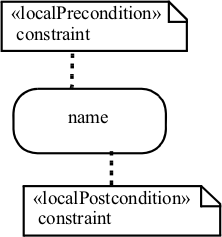
\includegraphics[scale=1]{./pics/local_postconditionsDiagram.PNG}
\end{figure}
\subsection{OCL}
\label{sec:OCL}


\section{Coverage Criteria}
\section{taxonomy of Model Based Testing}
Test Model,
Unit Test,
verdict,
Test data,
SUT,
Harness/ stubs,
declarative specification

\section{Preliminary Work}
\subsection{executing OCL}
A lot of research in the area of OCL and executing UML/OCL specifications has been performed by Matthias P. Krieger\cite{krieger2008executing}. Also Alloy and Dresden OCL or Eclipse OCL are projects that aim at executing and evaluating OCL specifications. 
\\
But solving OCL constraints as a CSP is only one part of generating test data from a UML Behaviour.
It is very common to use statemachines as the testmodel less papers are handling the generation of unit tests from UML Activities\cite{Linzhang04GeneratingTestCasefromActivityGrayBoxMethod}
\cite{Patel12TestCaseFormationUsigUMLActivityDiagram}
\cite{Pechtanun12GeneratingTestCaseFromUMLActivityDiagramBasedOnACGrammar}
\cite{Xu09ModelCheckingUMLActivities}\cite{Xu09ModelCheckingUMLActivityDiagramsFDR}. 


\subsection{Coverage Criteria}


\subsection{Generating Unit Tests}
Mark Uttig

Jeff Offut

Many papers suppose the use of state of the art SMT solvers such as HOL or CVC to solve OCL Postconditions, Preconditions and  of Operations and invariants embededto get possible inputvalues for functions that can be used as 
The only tool direktly targeted at generating Unit Tests form A UML specification with OCL constraints that was freely available was ParTeG by Stephan Weißleder. In his Ph.D thesis Stephan Weißleder describes a framework for applying different control flow based as well as partition based coverage criteria to state machines. He also develops a theory how all those coverage criteria are interconnected and can be simulated by each other and a transformed version of the original Test Model\cite{ParTeG}.


tell about other test generating tools (commercial, published in Papers) and ParTeG as the only one where the source code is available.\cite{ParTeG}

\section{The AMPL Modelling System}
\cite{AMPL}
